\documentclass[11pt,twocolumn]{article}
\usepackage{fullpage}
\usepackage{url}
\usepackage[margin=1.1in]{geometry}
\usepackage{graphicx}
\usepackage{csvsimple}
\begin{document}
\author{Ran Bernstein \\
\texttt{ranb@cs.technion.ac.il} \\
Department of Computer Science, Technion I.I.T, Haifa, Israel}
\title{Laban movement recognition from markerless motion capture sensor}
\maketitle
\begin{quote}{``Man moves in order to satisfy a need.`` ---\textup{Rudolph Laban}}
\end{quote}
\begin{abstract}
\textbf{Laban Movement Analysis (LMA), developed in the dance community
over the past seventy years, is an effective method for observing, describing, notating, and interpreting human
movement to enhance communication and expression in everyday and professional life.
Many applications that use motion capture data might be significantly
leveraged if the Laban qualities will be recognized automatically.
This paper presents an automated recognition method of Laban qualities from
motion capture skeletal recordings and it is demonstrated on the output of
Microsoft's Kinect V2 sensor.}
\end{abstract}
\section{Introduction}
\subsection{Laban movement analysis}
LMA is a formal language for motion description 
invented by Rudolf Laban \cite{Laban} in the middle of the 20th 
century. LMA describes, interprets and documents mental 
states from both conscious and unconscious human 
motion based on Laban�s theories of Body, Effort, Shape, 
and Space. LMA has been used in the fields of dancing, 
acting, athletics, physical therapy, and psychology and 
behavioral science. Laban exercises are based on the belief that by observing and analyzing 
movements, both conscious and unconscious, it is possible to recognize the objectives 
of the mover and to become aware of an inner attitude that precedes an action. Laban 
helps actors create momentary moods and long-standing personality characteristic 
through movement. For example, LMA work investigates the Effort properties -
Flow, Space, Time and Weight of all movement and helps actors think specifically about why their character may move in a jerky, fast, light and 
direct manner verses a heavy, slow, indirect and uninterrupted manner: 
\begin{itemize}
\item 
Flow: Bound or Free 
\item
Space: Direct or Indirect 
\item
Time: Sudden or Sustained 
\item
Weight: Strong or Light 
\end{itemize}
The whole hierarchy of LMA is described in figure number \ref{laban}.
\begin{figure*}[ht!]
\centering
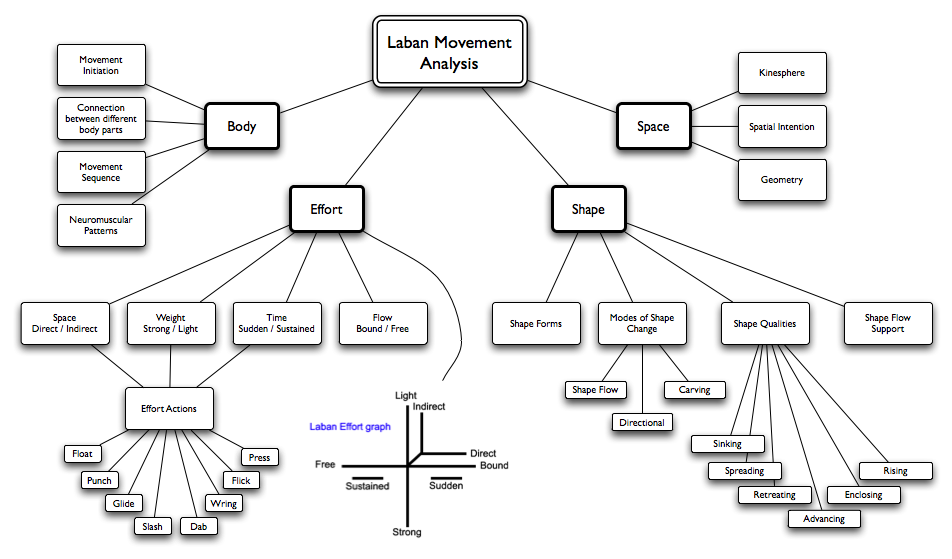
\includegraphics[width=\textwidth]{laban.png}
\caption{Laban movement analysis main axes.}
\label{laban}
\end{figure*}
\subsection{Laban qualities automated recognition}
Several attempts were made in order to recognize Laban qualities, most of them
were made for emotion recognition in the context of Human Robot Interaction (HRI).
Masuda et al. generated emotional body motion for a human 
form robot \cite{Masuda}. Rett et al. proposed a human motion recognition 
system using a Bayesian reasoning framework \cite{Rett}. Common in 
these studies, computational LMA offers some evidence that 
motion conveys emotional information, and this information 
allows such systems to estimate qualitative changes of motion.
Kim et al. performed first steps in this direction with the Kinect sensor, in 
this paper we extend such kind of work.
\subsection{Kinect sensor data}
This following figure shows the skeleton that is provided by the Kinect's
software development kit that were use in this paper.
\begin{figure}[ht!]
\centering
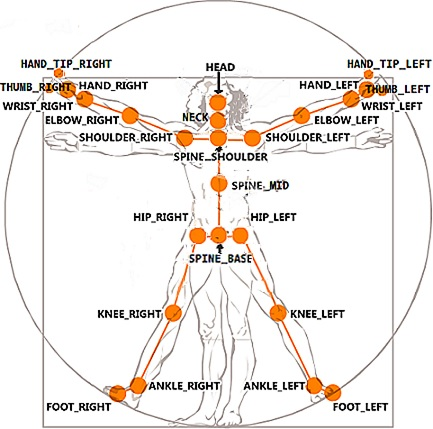
\includegraphics[width=60mm]{skeleton.jpg}
\caption{Skeleton positions relative to the human body}
\label{skeleton}
\end{figure}
Once the skeleton is detected, the 3D coordinates of all joints of user�s body 
� with the exception of joints, that are not visible (e.g. a user�s hand is
behind his back) are provided.
As seen in figure \ref{Coordinate}, the coordinates are in a �real-world�
coordinate system, that has the beginning [0,0,0] in the sensor, x,y and z-axis goes as shown on the picture below and the units are milimeters. 
\begin{figure}[ht!]
\centering
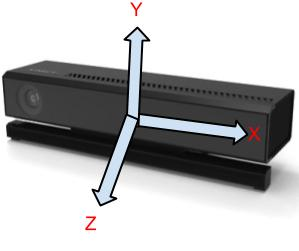
\includegraphics[width=60mm]{KinectV2CoordinateSystem.jpg}
\caption{Kinect Coordinate System}
\label{Coordinate}
\end{figure}
\section{Method}
\subsection{Dataset collection}
The dataset was created by recording 5 Certified Movements Analysts (CMA)
performing random movements with several Laban qualities. Every clip is about
3 seconds long that were captured by the Kinect.
here goes table with an elaboration about the amount of every quality every 

\subsection{Feature Extraction}
Due to unequal length of clips, all the features that were extracted are in
whole clip granularity.
\subsubsection{General low level features}
For every joint in the skeleton the angular velocity, acceleration and jerk were
extracted, and for each one of them the mean, variance, skew and kurtosis were
extracted (the extraction of the last four moments is denoted as \phi). 
\subsubsection{Shape: Sagital}
In this quality a separation between Advance and Retreat. The quantification of
this quality was done by projecting the speed vector of the Center Of Mass (COM)
on the vector of the front of the body. The COM was approximated in this case
by the average of all of the joints. The front of the body was approximated by
the perpendicular vector to the the vector between the Left Shoulder (LS) and
the Right Shoulder (RS).
\\If $\vec{P}_{j}(t)$ is the vector of the position of joint j in time t in
a clip with n frames, and $ \alpha_{j}$ is a coefficient proportional to the
mass around of the joint:
\\
\\\vec{P}_{COM}(t) = \sum_{j \in Joints} \alpha_{j}\vec{P}_{j}(t)
\\
\\\vec{P}_{shoulders}(t)=\vec{P}_{LS}(t)-\vec{P}_{RS}(t)
\\
\\\vec{P}_{front}=\vec{P}_{shoulders}\[ \left( \begin{array}{ccc}
0 & 0 & 1 \\
0 & 1 & 0 \\
-1 & 0 & 0 \end{array} \right)\] 
\\
\\S_{sag}(t) = \vec{P}_{COM}(t)\cdot\vec{P}_{front}(t)
\\
\\\vec{F}_{sag} = \phi([S_{sag}(1), \ldots S_{sag}(n)])
\\\\
Where $ \phi$ is the moments extraction.
\subsubsection{Shape: Horizontal}
Here the separation is between spreading and enclosing in the horizontal axe.
This quality was quantified by measuring the average distance of the joint from
the the vertical axe of the body that spreads from the Head (H) along the Spine
Base (SB).
This axe was approximated with the Kinect's horizontal axe(y), what made the
distance measured in the projection of the joints on the XZ plane.
\\
\\d_{j} = \frac{\left|(\vec{P}_{j}-\vec{P}_{SB})\times
(\vec{P}_{j}-\vec{P}_{H})\right|}{\left|\vec{P}_{H}-\vec{P}_{SB}\right|}
\\
\\S_{horiz}(t) = \sum_{j \in Joints} d_{j}(t)
\\
\\\vec{F}_{horiz} = \phi([S_{sag}(1), \ldots S_{sag}(n)])
\\\\
Where $ \phi$ is the moments extraction.
\subsubsection{Shape: Vertical}
Here the separation is between Rise and sink.
This quality was quantified by measuring the average distance on axe y of each
joint from the COM. This quantification comes from the assumption that the body
is ``longer'' when rising.
\\
\\S_{vert}(t) = \sum_{j \in Joints}
\left|\vec{P}_{j}-\vec{P}_{COM}\right|
\\
\\\vec{F}_{vert} = \phi([S_{sag}(1), \ldots S_{sag}(n)])
\\\\
Where $ \phi$ is the moments extraction.
\subsubsection{Effort: Time}
Here the separation is between Sudden or Sustained. This quality was 
quantified by the skew of the acceleration, relaying on the belief that the
acceleration of a sudden movement will be more left skewed in the the beginning
of the movement (where the acceleration is positive).
\subsubsection{Effort: Space}
Here the separation is between direct and indirect. This quality was 
quantified by the angle between the movement vector of a joint to the next one,
relaying on the belief that in direct movement every vector will be in
the same direction as the last (the angle between them is small).
\\If $\vec{P}_{j}(t)$ is the vector of the position of joint j in time t, the
movement vectors are:
\\\\\vec{V}_{j}(t) = \vec{P}_{j}(t+1) - \vec{P}_{j}(t)
\\\\$The angles between them are calculated with inner products:$
\\\\\vec{A}_{j}(t) = \vec{V}_{j}(t+1) \cdot \vec{V}_{j}(t)


\subsection{Performance Evaluation}
There are about 40 labels (Laban qualities) that every recording can get, but
a typical gesture usually includes about 3 qualities, what means that there is
more than 90\% chance that a quality won't characterize the gesture. Due to
this sparsity, a simple accuracy is not a relevant metric for the performance
evaluation because one can get 90\% accuracy by stating that for every recording
non of the qualities appear. A better evaluation have to combine the precision
and recall rates of the classifier. The way that the last two were combined is
with the usage of F one score:
\\
\\F_{1} = \frac{2\cdot precision\cdot recall}{precision+recall}
\subsection{Feature Selection}
The extraction of every recording into a vector created long
vectors of about 10000 features, most of are noisy. For that reason a
massive features selection were needed. The features selection was done by
computing the Anova F-value for every feature over the training set. Cross
validation was used to determine the optimal amount of features that should be
left. As it seen in figure  \ref{selection}, The result was that the filtering
of the vectors outperformed the usage in non filtered vectors, where using the top 5\% of features was optimal.
\begin{figure}[ht!]
\centering
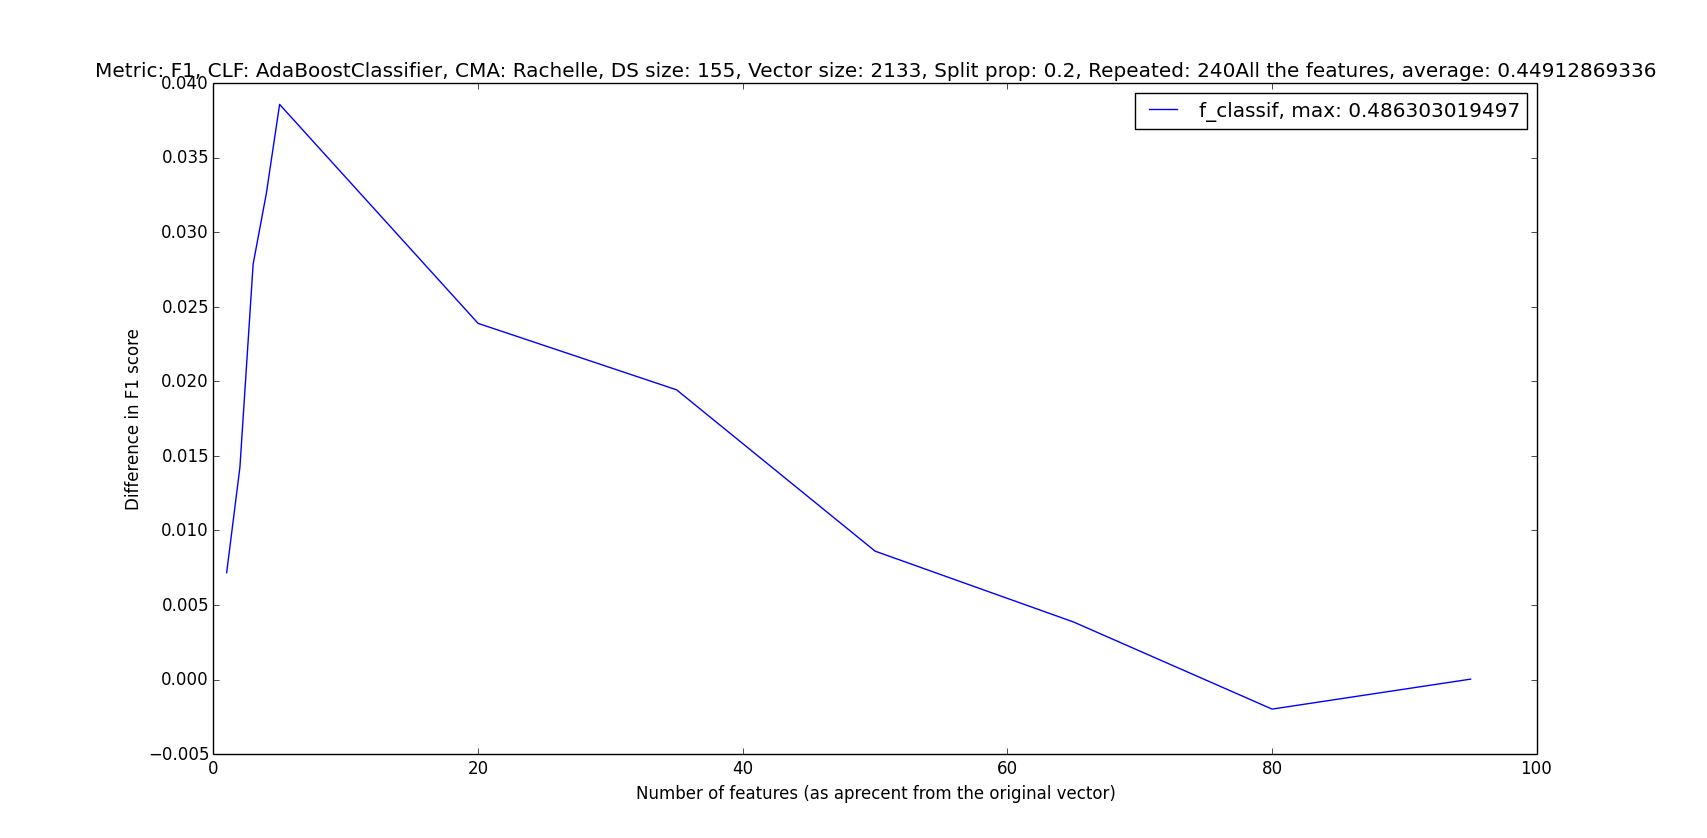
\includegraphics[width=60mm]{featureSelection.png}
\caption{Influence of the percent of features that were used on the F1 score.
The blue line is the difference between the score with an without feature
selection. It can be seen that the optimal amount to slecet is 5\%}
\label{selection}
\end{figure}

\subsection{Multi-label classification}
Multi-label learning deals with the problem where each instance is associated
with multiple labels simultaneously, where the number of labels is not fixed
between instance to instance. The task of this learning paradigm is to predict
the label (Laban quality) set for each unseen instance (skeletal recording), 
through analyzing training instances with known label sets. The algorithm that
was used is Adaboost with decision tree as the week classifier. In every run on
a data set it was splitted to 80\%/20\% to train and test sets respectively.
\section{Results}
\subsection{Experiment 1}
In this experiment both of the train and test datasets are taken from the same
CMA.
\begin{figure*}[ht!]
\centering
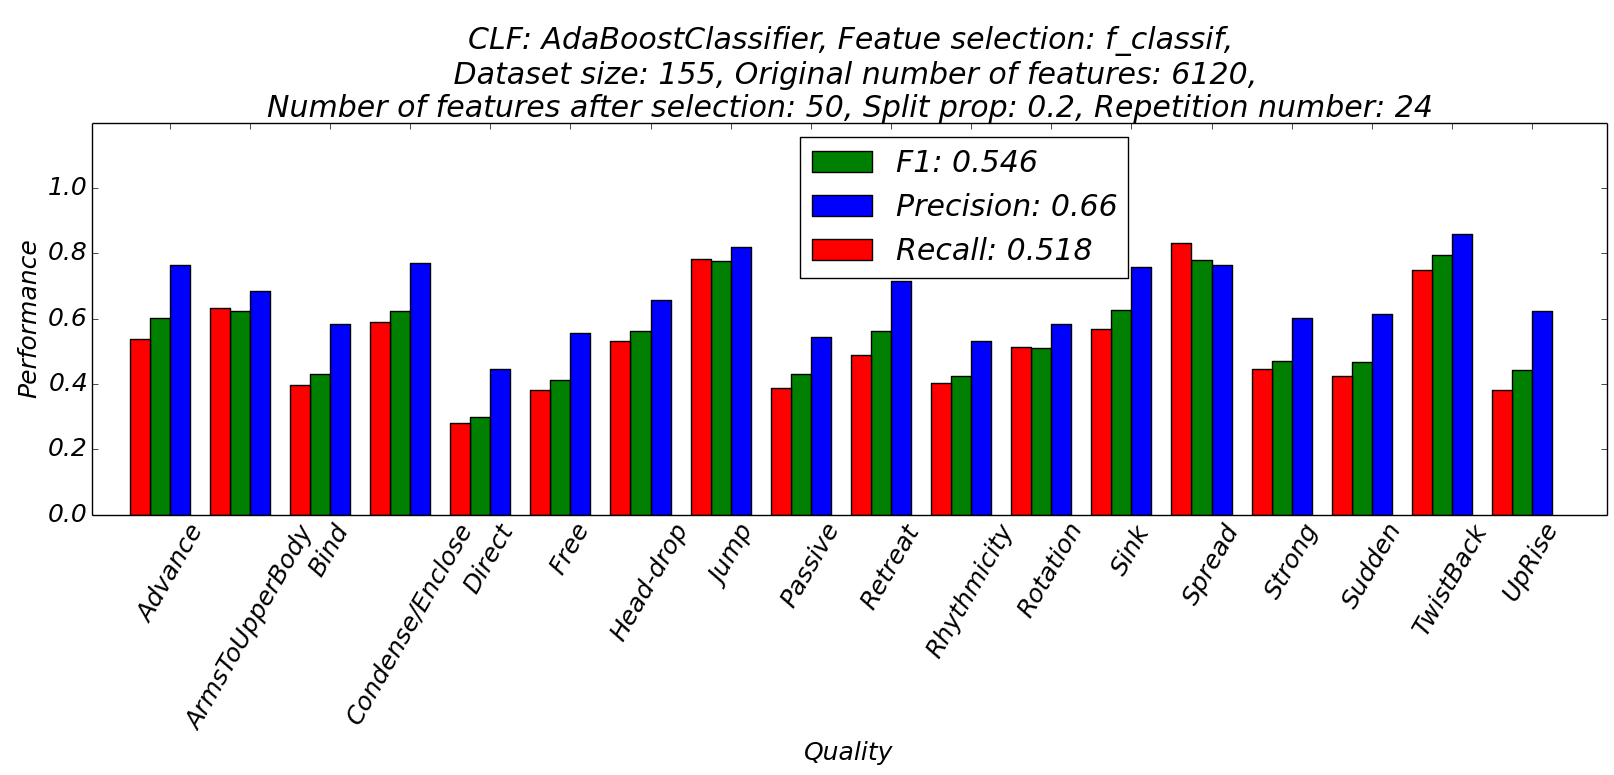
\includegraphics[width=\textwidth, height=60mm]{qualities.png}
\caption{Recall, precision and F1 score of each Laban quality separately.}
\label{qualities}
\end{figure*}

\subsection{Experiment 2}
In this experiment the train set was taken from one CMAm while the test set
was taken from another. The precision, recall and F1 scores where 0.57, 
0.42 and 0.43 respectivaly. The best features are represented in table
 \ref{bestFeatures}.
\begin{figure*}[ht!]
\centering
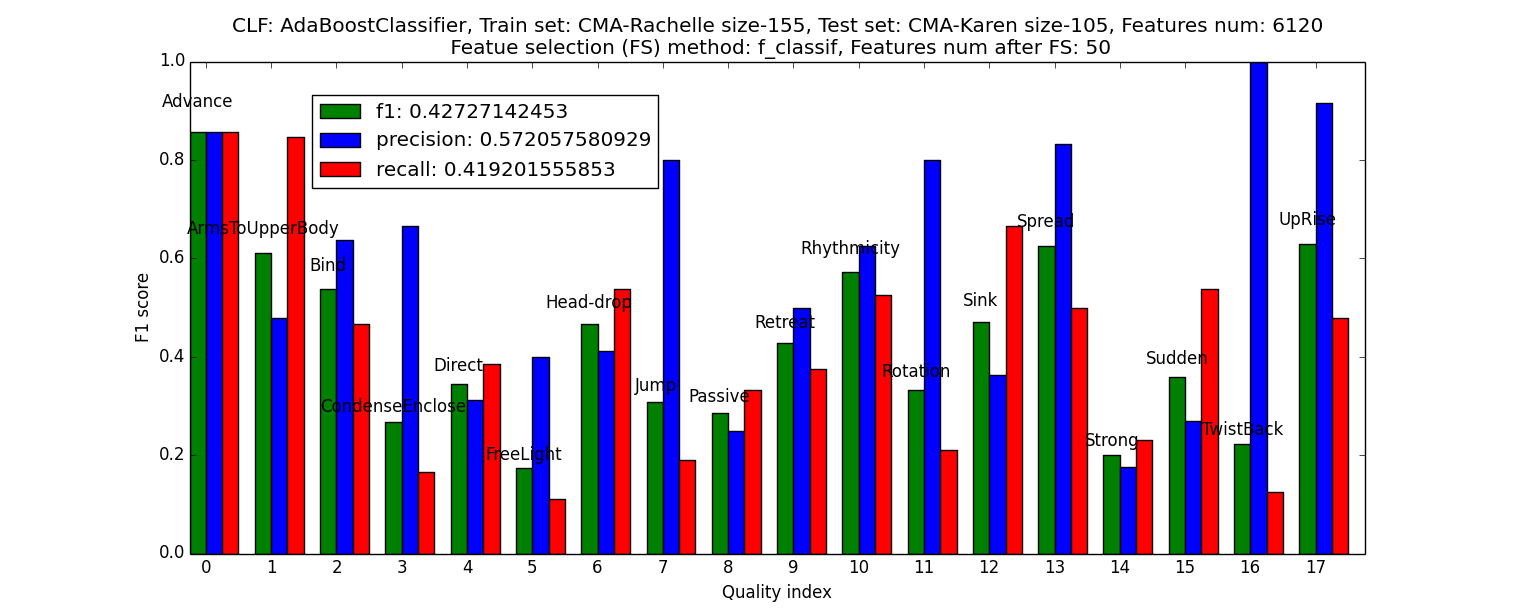
\includegraphics[width=\textwidth, height=60mm]{Rachelle2Karen.png}
\caption{Recall, precision and F1 score of each Laban quality where the train
set is from one CMA and the test set is from another. F1 one score is 0.43}
\end{figure*}
\begin{document}
\begin{table*}
   \centering
   \csvautotabular{bestFeatures.csv}
   \caption{The feature with the highest F-value for every quality}
   \label{bestFeatures}
\end{table*}

\begin{table*}
   \centering
   \csvautotabular{performance.csv}
   \caption{Recall, precision and F1 score of each Laban quality where the train
set is from one CMA and the test set is from another. Average F1 one score is
0.43}
   \label{bestFeatures}
\end{table*}

\subsection{Experiment 3}
In this experiment the datasets of the two CMAs were mixed, and from the
mixture both of the train and test sets were taken.
\begin{figure*}[ht!]
\centering
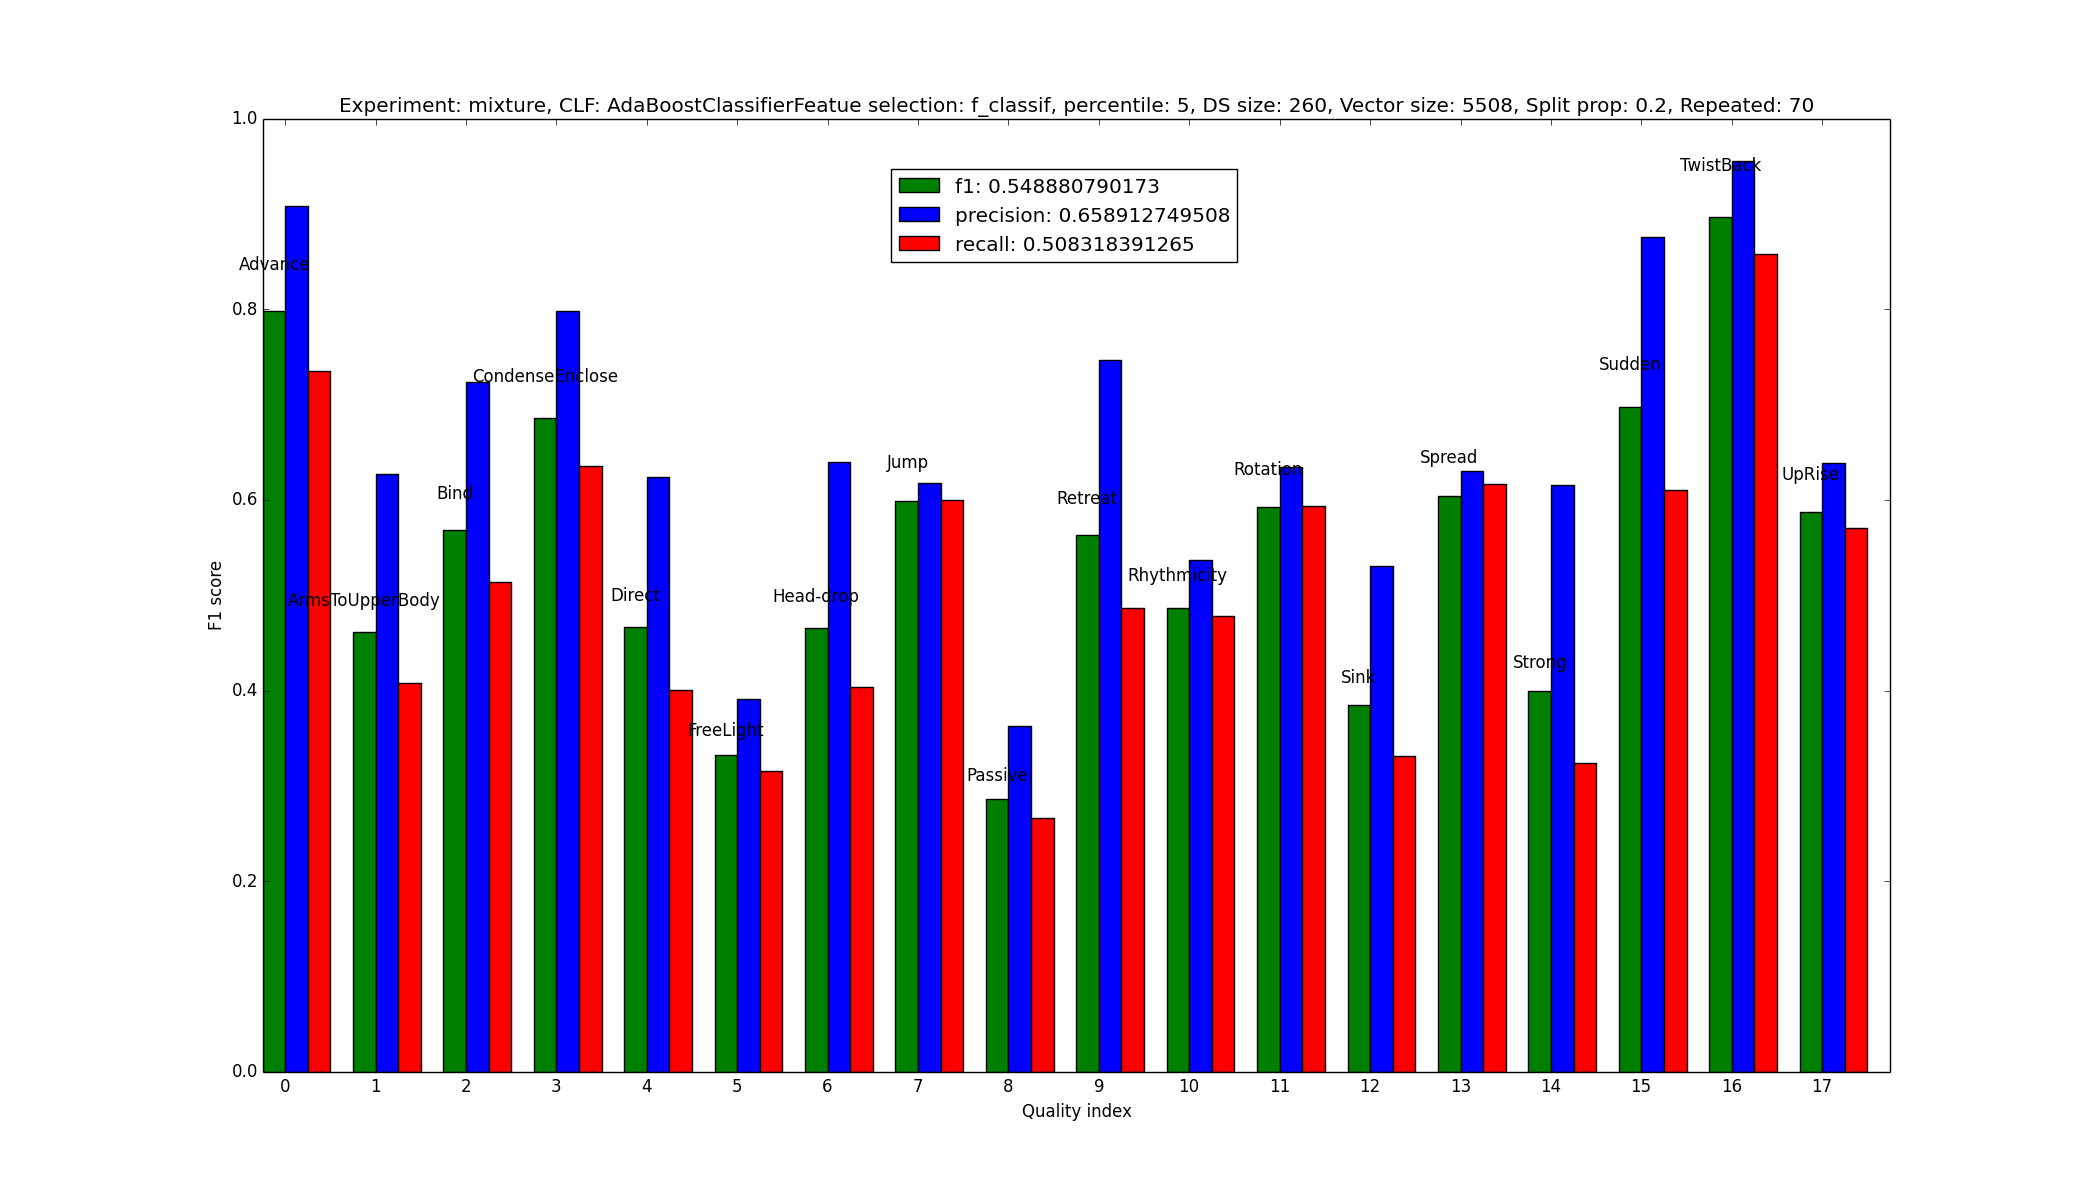
\includegraphics[width=\textwidth, height=60mm]{mixture.png}
\caption{Recall, precision and F1 score of each Laban quality where the train
set is from one CMA and the test set is from another. F1 one score is 0.37}
\label{qualities}
\end{figure*}
\begin{thebibliography}{1}
\bibliographystyle{alpha}
  \bibitem{Bouchard}Bouchard, Durell, and Norman Badler. "Semantic segmentation
  of motion capture using laban movement analysis." Intelligent Virtual Agents. Springer Berlin Heidelberg, 2007. 
  \bibitem{Camurri}Antonio Camurri, Giovanni De Poli, Anders Friberg, Marc Leman
	& Gualtiero Volpe (2005): The MEGA Project: Analysis and Synthesis of
	Multisensory Expressive Gesture in Performing Art Applications, Journal of New
	Music Research, 34:1, 5-21
	\bibitem{Castellano}Ginevra Castellano , Santiago D. Villalba , Antonio
	Camurri, Recognising Human Emotions from Body Movement and Gesture Dynamics, 
	Proceedings of the 2nd international conference on Affective Computing and Intelligent Interaction, 
	September 12-14, 2007, Lisbon, Portugal  
  \bibitem{Chen}Chen, J., et al. "Analysis and evaluation of human
  movement based on laban movement analysis." Tamkang Journal of Science and Engineering 13.3 (2011): 255-264. 
  \bibitem{Foroud}Foroud, Afra, and Ian Q. Whishaw. "The consummatory origins of
  visually guided reaching in human infants: a dynamic integration of whole-body and upper-limb movements." Behavioural brain research 231.2 (2012): 343-355. \bibitem{Karpouzis}Karpouzis, Kostas, 
  et al. "Modeling naturalistic affective
  states via facial, vocal, and bodily expressions recognition." Artificial intelligence for human computing. Springer Berlin Heidelberg, 2007. 91-112. 
  \bibitem{Garber}Garber-Barron, Michael, and Mei Si. "Using body movement and
  posture for emotion detection in non-acted scenarios." Fuzzy Systems (FUZZ-IEEE), 2012 IEEE International Conference on. IEEE, 2012. \bibitem{Kim}Kim, Woo Hyun, et al. "LMA based emotional motion representation
  using RGB-D camera." Proceedings of the 8th ACM/IEEE international conference on Human-robot 
  interaction. IEEE Press, 2013.
  \bibitem{Laban} Laban, Rudolf, and Lisa Ullmann. "The mastery of movement."
  (1971).
  \bibitem{Lourens}Lourens, Tino, Roos Van Berkel, and Emilia Barakova.
  "Communicating emotions and mental states to robots in a real time parallel framework using Laban movement analysis." Robotics and Autonomous Systems 58.12 (2010): 1256-1265. 
  \bibitem{Masuda}M. Masuda and S. Kato, �Motion Rendering System for 
	Emotion Expression of Human Form Robots Based on Laban 
	Movement Analysis,� 19th IEEE International Symposium on 
	Robot and Human Interactive Communication, Italy, 2010. 
  \bibitem{Nguyen}Nguyen, Anh-Tuan, Wei Chen, and Matthias Rauterberg. "Online
  Feedback System for Public Speakers." IEEE Symp. e-Learning, e-Management and e-Services. 2012. \bibitem{Rett}J. Rett and J. Dias, �Bayesian reasoning for Laban Movement
  Analysis used in human-machine interaction,� International Journal of Reasoning-based 
  Intelligent Systems, Vol. 2, No. 1,pp. 13-35, 2010
  \bibitem{Savva}Savva, Nikolaos, Alfonsina Scarinzi, and Nadia
  Bianchi-Berthouze. "Continuous recognition of player's affective body expression as dynamic quality of aesthetic experience." 
  Computational Intelligence and AI in Games, IEEE Transactions on 4.3 (2012): 199-212. 
  \bibitem{Zacharatos}Zacharatos, Haris, et al. "Emotion Recognition for Exergames
  using Laban Movement Analysis." Proceedings of the Motion on Games. ACM, 2013.
   
 \end{thebibliography}
\end{document}
